\documentclass{article}
\usepackage[utf8]{inputenc}
\usepackage{amsfonts, amsmath, amssymb, amsthm}
\usepackage{geometry}
\usepackage{enumitem}
\usepackage{hyperref}
\usepackage{pgfplots}
\usepackage{parskip}
\usepackage{graphicx}
\usepackage{caption, subcaption}
\usepackage{xcolor}

%%%%%%%%%%%%%%%%%%%%%%%%%%%%%%%%%%%%%%%%%%%%%%%%%%%%%%%%%%%%%%%%%%%%%%%%%%%%%%%%%%%%%%%%%%%%%%%%%%%%%%%%%%%%%%%%%%%%%%%%%%%%

\newtheorem{theorem}{Theorem}
\newtheorem{example}[subsubsection]{Example}

%%%%%%%%%%%%%%%%%%%%%%%%%%%%%%%%%%%%%%%%%%%%%%%%%%%%%%%%%%%%%%%%%%%%%%%%%%%%%%%%%%%%%%%%%%%%%%%%%%%%%%%%%%%%%%%%%%%%%%%%%%%%

\newcommand{\bluelink}[2]{{\color{blue}\underline{\href{#1}{#2}}}}
\newcommand{\reference}[2]{{\color{blue}\underline{\href{#1}{\textit{#2}}}}}
\newcommand{\R}{\mathbb{R}}
\newcommand{\point}{(x_0, y_0)}
\newcommand{\del}{\partial}
\newcommand{\grad}{\vec{\nabla}}
\newcommand{\ddvp}{(\ddv)_{P_0}}
\newcommand{\ddv}{D_{\hat{u}}f}
\newcommand{\llangle}{\left\langle}
\newcommand{\rrangle}{\right\rangle}

%%%%%%%%%%%%%%%%%%%%%%%%%%%%%%%%%%%%%%%%%%%%%%%%%%%%%%%%%%%%%%%%%%%%%%%%%%%%%%%%%%%%%%%%%%%%%%%%%%%%%%%%%%%%%%%%%%%%%%%%%%%%

\graphicspath{{./Images/}}
\geometry{a4paper, left=25mm, right=25mm, top=25mm, bottom=25mm}

%%%%%%%%%%%%%%%%%%%%%%%%%%%%%%%%%%%%%%%%%%%%%%%%%%%%%%%%%%%%%%%%%%%%%%%%%%%%%%%%%%%%%%%%%%%%%%%%%%%%%%%%%%%%%%%%%%%%%%%%%%%%

\title{
    MTH203: Multivariate Calculus (Math-III) \\
    \Large Monsoon Semester, 2022
}
\author{Indraprastha Institute of Information Technology, Delhi}
\date{}

%%%%%%%%%%%%%%%%%%%%%%%%%%%%%%%%%%%%%%%%%%%%%%%%%%%%%%%%%%%%%%%%%%%%%%%%%%%%%%%%%%%%%%%%%%%%%%%%%%%%%%%%%%%%%%%%%%%%%%%%%%%%

\begin{document}
\maketitle

%%%%%%%%%%%%%%%%%%%%%%%%%%%%%%%%%%%%%%%%%%%%%%%%%%%%%%%%%%%%%%%%%%%%%%%%%%%%%%%%%%%%%%%%%%%%%%%%%%%%%%%%%%%%%%%%%%%%%%%%%%%%

% Introduction
\section*{About the Instructor}
\textbf{Name:} \bluelink{mailto:sarthok@iiitd.ac.in}{Sarthok Sircar}

\textbf{Office Hours:} By appointment

\section*{About the Course}
\textbf{Course Code and Name:} MTH203: Multivariate Calculus (Math-III)

\textbf{Prerequisites:} None

\textbf{Anti-requisites:} MTH240: Real Analysis-I

\textbf{Description:}

This course covers topics in multivariable calculus, vector calculus, and complex analysis. The course starts with an
extension of concepts like limits, continuity, and differentiation to functions of multiple variables. Partial
differentiation is defined and applied. The idea of Taylor series is extended to functions of two variables. This is
followed by a definition and application of integration in more than one dimensions, i.e. double and triple integrals. We
then work with vector functions and develop the ideas of vector fields and differentiation and integration as applicable to
vector calculus (gradient, divergence, curl, line and surface integrals, etc.) The ideas of circulation and flux are
developed and Green's, Stoke's and divergence theorems are covered. The final module of the course deals with complex
numbers and functions and an extension of concepts of calculus to complex variables.

\textbf{Grading Scheme:}
\begin{enumerate}
    \item \textbf{30\%}: 12 Assignments/Worksheets to be solved in tutorials. Out of 12, best 10 assignments will be
    considered for grading, making each assignment worth 3\%.

    \item \textbf{35\%}: 1 Mid-Sem Exam.
    \item \textbf{35\%}: 1 End-Sem Exam.
\end{enumerate}

\textbf{Important Links:}
\begin{enumerate}
    \item \bluelink{http://techtree.iiitd.edu.in/viewDescription/filename?=MTH203}{Course Directory}
    \item \bluelink{https://classroom.google.com/c/NDA4NDczODQwNTla}{Google Classroom}
\end{enumerate}

\pagebreak

%%%%%%%%%%%%%%%%%%%%%%%%%%%%%%%%%%%%%%%%%%%%%%%%%%%%%%%%%%%%%%%%%%%%%%%%%%%%%%%%%%%%%%%%%%%%%%%%%%%%%%%%%%%%%%%%%%%%%%%%%%%%

% Multivariable Functions
\section{Multivariable Functions}

\subsection{Functions in two variables}
Let $X \subseteq \R$ and $Y \subseteq \R$. If for every $(x, y) \in X \times Y, \exists \text{ a unique } z \in \R$
according to some rule $z = f(x, y)$, then $f(x, y)$ is said to be a real-valued function in two variables, $x$ and $y$, given by
\begin{equation}
    z = f(x, y),\ (x, y) \in X \times Y
\end{equation}

The variables $x$ and $y$ are $independent$ and $z$ is $dependent$ (on $x$ and $y$).


\subsection{Functions in \texorpdfstring{$n$}{n} variables}
In general, let $T \in \R^n$. A real valued function $f$ on $T$ is a rule that assigns a $w \in \R$ such that
\begin{equation}
    w = f(x_1, x_2, x_3, \hdots, x_n),\ x_i \in \R\ \forall i \in \{1, 2, 3, \hdots, n\}
\end{equation}

for all elements in $T$. Here, the variables $x_1, x_2, x_3, \hdots, x_n$ are $independent$ and $w$ is $dependent$.

%%%%%%%%%%%%%%%%%%%%%%%%%%%%%%%%%%%%%%%%%%%%%%%%%%%%%%%%%%%%%%%%%%%%%%%%%%%%%%%%%%%%%%%%%%%%%%%%%%%%%%%%%%%%%%%%%%%%%%%%%%%%

% Types of Points and Regions
\section{Types of Points and Regions}

\subsection{Types of Points}
A point $\point$ in a region $S$ in the $xy$-plane is called:

\begin{enumerate}
    \item An \textbf{Interior Point} if there exists a disc centered at $\point$ that lies entirely in $S$.

    \item A \textbf{Boundary Point} if every disc centered at $\point$ contains some points that lie inside $S$ and some
    points that lie outside $S$.

    \item An \textbf{Exterior Point} if it is neither an \textbf{Interior Point} nor a \textbf{Boundary Point}.
\end{enumerate}

\begin{figure}[htp]
    \centering
    \begin{tikzpicture}
        \begin{axis}[
            axis lines = middle,
            axis equal,
            xmin=-1.5, xmax=1.5, ymin=-1.5, ymax=1.5,
            xlabel = $x$,
            ylabel = $y$,
            xticklabels = {,,},
            yticklabels = {,,},
            title = {Interior, Exterior, and Boundary Points}]

            \draw (axis cs: 0, 0) circle [radius=100];
            \addplot[scatter, only marks] coordinates{(0.45, 0.45) (-1, 0) (1, -1)};
            \draw (axis cs: 0.45, 0.45) circle [radius=15];
            \draw (axis cs: -1, 0) circle [radius=15];
            \draw (axis cs: 1, -1) circle [radius=15];
        \end{axis}
    \end{tikzpicture}
    \caption{$S = \{(x, y) \in \R^2\ |\ x^2 + y^2 = 1\}$}
\end{figure}


\subsection{Types of Regions}
A region is said to be:

\begin{enumerate}
    \item \textbf{Open} if it ONLY contains interior points.
    \item \textbf{Closed} if along with all interior points, it also contains ALL boundary points.
    \item \textbf{Bounded} if it can be enclosed within a disc of (fixed) finite radius.
    \item \textbf{Unbounded} if it cannot be enclosed within a disc of finite radius.
\end{enumerate}


\subsection{Examples}

\begin{example}
    \normalfont
    Open unit disc: $S = \{(x, y) \in \R^2\ |\ x^2 + y^2 < 1\}$
\end{example}

\begin{example}
    \normalfont
    Boundary of unit disc: $S = \{(x, y) \in \R^2\ |\ x^2 + y^2 = 1\}$
\end{example}

\begin{example}
    \normalfont
    Closed unit disc: $S = \{(x, y) \in \R^2\ |\ x^2 + y^2 \leq 1\}$
\end{example}

\begin{example}
    \normalfont
    \textbf{Bounded Regions:} Circles, Ellipses, Rectangles, etc.
\end{example}

\begin{example}
    \normalfont
    \textbf{Unbounded Regions:} Parabolas, Hyperbolas, Planes, etc.
\end{example}

%%%%%%%%%%%%%%%%%%%%%%%%%%%%%%%%%%%%%%%%%%%%%%%%%%%%%%%%%%%%%%%%%%%%%%%%%%%%%%%%%%%%%%%%%%%%%%%%%%%%%%%%%%%%%%%%%%%%%%%%%%%%

% Level Curves, Graphs, and Surfaces
\section{Level Curves, Graphs, and Surfaces}
\begin{enumerate}
    \item \textbf{Level Curve and Level Surface} \\
    The set of points in the plane where a function $f(x, y)$ has a constant value, i.e. where $f(x, y) = c$
    is called a \textbf{level curve} of $f$. In essence, the set of all points $(x, y, z) \in \R^3$, where
    a function of the \textit{independent} variables has a constant value $z = f(x, y) = c$ is called the
    \textbf{level surface} of $f$.

    \item \textbf{Graph or Surface} \\
    The set of all points $(x, y, f(x, y)) \in \R^3$ for $(x, y)$ in the domain of $f$ is called the
    \textbf{graph} or \textbf{surface} of $f$.

    \item \textbf{Contour Curve} \\
    A plane $z = c$ cuts the surface $z = f(x, y)$ in the points given by $f(x, y) = c$. This curve in space
    is called the \textbf{contour curve} $f(x, y) = c$. The contour curve is a curve in the plane $z = c$,
    whereas the level curve is a curve in the $xy$-plane.
\end{enumerate}

\textbf{Reference Link:}
\reference{https://www.youtube.com/watch?v=acdX4YamDtU}{Visualizing Multi-variable Functions with Contour Plots}

\begin{figure}[h]
    \begin{subfigure}[b]{0.5\textwidth}
        \centering
        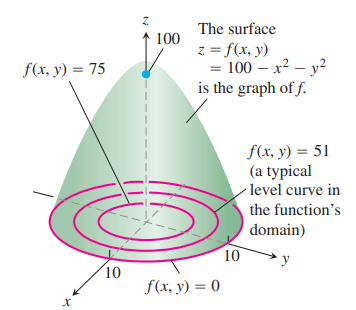
\includegraphics[scale=0.85]{level-curve-1.png}
        \caption{Level Curves}
    \end{subfigure}
    \hfill
    \begin{subfigure}[b]{0.5\textwidth}
        \centering
        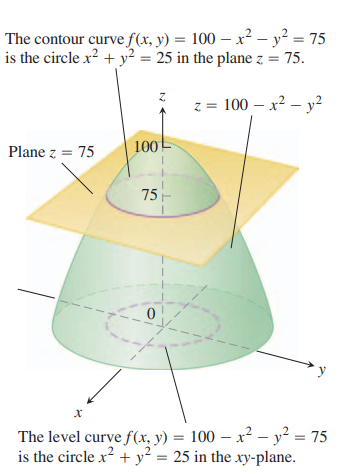
\includegraphics[scale=0.75]{contour-curve-1.png}
        \caption{Contour Curves}
    \end{subfigure}
\end{figure}

\begin{example}
    \normalfont For the plane $z = 50$ on the surface of $z = 75 - x^2 - y^2$:
    \begin{enumerate}
        \item The contour curve is the circle $x^2 + y^2 = 25$ in the plane $z = 50$.
        \item The level curve is $f(x, y) = 75 - x^2 - y^2 = 50$, i.e. the circle $x^2 + y^2 = 25$ in the $xy$-plane.
    \end{enumerate}
\end{example}

%%%%%%%%%%%%%%%%%%%%%%%%%%%%%%%%%%%%%%%%%%%%%%%%%%%%%%%%%%%%%%%%%%%%%%%%%%%%%%%%%%%%%%%%%%%%%%%%%%%%%%%%%%%%%%%%%%%%%%%%%%%%

% Limits
\section{Limits}

\subsection{Limits of functions in one variable}
Recap, the limit of a function $f(x)$ at $x = x_0$ is given by:
\begin{equation}
    \lim_{x \to x_0} f(x) = L
\end{equation}
i.e., as $x$ \textit{approaches} $x_0$, $f(x)$ \textit{approaches} $L$.


\subsection{Limits of functions in two variables}
The limit of a function $f(x, y)$ at a point $\point \in \R^2$ is given by:
\begin{equation}
    \lim_{(x, y) \to \point} f(x, y) = L
\end{equation}
i.e., as $(x, y)$ \textit{approaches} $\point$, $f(x, y)$ \textit{approaches} $L$. The same concept of limit
in \textit{one} dimiensions is easily generalized to higher dimensions, taking care of the fact that in higher
dimensions, there are more ways to \textit{approach} a point.


\subsection{The \texorpdfstring{$\epsilon$-$\delta$}{e-d} definition of a limit}
(In general) The limit of a function $f(x, y)$ as $(x, y)$ approaches $\point$ is equal to $L$ if for every $\epsilon > 0$,
there exists a corresponding $\delta \in \R^+$, such that for all $x$
\begin{equation}
    |f(x, y) - L| < \epsilon \text{ whenever } \lVert (x, y) - \point \rVert < \delta
\end{equation}

\begin{example}
    \normalfont Find the limit of $f(x, y) = 2x + y$ at the point $(1, 2)$ using the $\epsilon$-$\delta$
    definition of the limit.

    We need to find:
    $$\lim_{(x, y) \to (1, 2)} (2x + y) = ?$$
    Assuming the limit exists, let $\epsilon > 0$ be some real value. Let $L = f(1, 2) = 4$. We need to make sure that
    $$|2x + y - 4| < \epsilon \text{ whenever } \lVert(x, y) - (1, 2) \rVert = \sqrt{(x-1)^2 + (y-2)^2} < \delta$$
    \begin{align*}
        |2x + y - 4| &= |2 (x-1) + y - 2| \\
        &\leq |2 (x-1)| + |y - 2| \\
        &\leq 3 \delta
    \end{align*}
    If we take $\delta = \epsilon/3$, then $|2x + y - 4| < \epsilon$ whenever $|x - 1| < \delta$ and $|y - 2| < \delta$.
    Hence, the limit exists and is equal to 4.
\end{example}


\subsection{Properties of limits}
\begin{enumerate}
    \item The limit of a function $f(x, y)$ at a point $\point \in \R^2$ if exists, is unique.

    \item Substituting $x - x_0 = r\cos{\theta}$ and $y - y_0 = r\sin{\theta}$ where $r^2 = (x - x_0)^2 + (y - y_0)^2$
    and $\text{tan}\theta = \frac{x - x_0}{y - y_0}$, the definition of the limit can be expressed as:

    $\forall \epsilon > 0,\ \exists\ \delta > 0$, such that $\forall\ (r, \theta) \in \R^2,\ |r| > \delta \implies$
    $|f(r\cos{\theta}, r\sin{\theta}) - L| < \epsilon$

    \begin{example}
        \normalfont Prove that: $$\lim_{(x, y) \to (0, 0)} \left( \frac{x^3}{x^2 + y^2} \right) = 0$$

        Let $x = r\cos{\theta}$ and $y = r\sin{\theta}$. Then,
        $$\lim_{r \to 0} r\sin^3{\theta} = 0,\ \forall \ \theta \in \R$$
        So, let $L = 0$ and $\epsilon > 0$ such that:
        \begin{align*}
            |r\cos^3{\theta} - 0| &\leq |r| < \delta \\
            \text{and }|r\cos^3{\theta} - 0| &\leq \epsilon \text{ whenever } |r| < \delta \\
            \left| \frac{x^3}{x^2 + y^2} \right| = |x| \left| \frac{x^2}{x^2 + y^2} \right| \leq |x| &\leq \epsilon \text{ whenever }
            \sqrt{x^2 + y^2} < \delta
        \end{align*}
        So, $|f(x, y) - 0| \leq \delta$. Hence, proved.
    \end{example}

    \item \textbf{The two path test for non-existence of a limit} \\
    If the function $f(x, y)$ takes different values as $(x, y)$ approaches $\point$ from different paths, then the limit
    of $f(x, y)$ at the point $\point$ does not exist.

    \item \textbf{Path independence of limit} \\
    If the limit of a function $f(x, y)$ at a point $\point \in \R^2$ exists, then regardless of the path from which $(x, y)$
    approaches $\point$, the function takes the same value.

    \begin{example}
        \normalfont Find the limit:
        $$\lim_{(x, y) \to (0, 0)} \left( \frac{xy}{x^2 + y^2} \right)$$

        Along the $x$-axis, $y = 0$; the $y$-axis, $x = 0$; and the path $y = x$, we have (respectively):
        $$\lim_{y \to 0} \frac{0}{x^2} = \lim_{x \to 0} \frac{0}{y^2} = 0 \neq \lim_{x \to 0} \frac{x^2}{2x^2} = \frac{1}{2}$$
        Hence, the limit does not exist.
    \end{example}

    \item If the (two-dimensional) limit $\lim_{(x, y) \to \point} f(x, y) = L$
    exists, then the (iterated) limits
    $$\lim_{x \to x_0}\left( \lim_{y \to y_0} f(x, y) \right) \text{ and } \lim_{y \to y_0}\left( \lim_{x \to x_0} f(x, y) \right)$$
    exist, and are equal to $L$, provided the (one-dimensional) limits exist.
\end{enumerate}

%%%%%%%%%%%%%%%%%%%%%%%%%%%%%%%%%%%%%%%%%%%%%%%%%%%%%%%%%%%%%%%%%%%%%%%%%%%%%%%%%%%%%%%%%%%%%%%%%%%%%%%%%%%%%%%%%%%%%%%%%%%%

% Continuity
\section{Continuity}

\subsection{Definition of continuity}
A function $f(x, y)$ is said to be \textit{continuous} at a point $\point \in \R^2$ if:
\begin{enumerate}
    \item $f$ is defined at $\point$.
    \item $\lim_{(x, y) \to \point} f(x, y) = f\point$
\end{enumerate}

\begin{example} \normalfont Find out whether the given function is continuous:
    \begin{equation*}
        f(x, y) =
        \begin{cases}
            \frac{(x - y)^2}{x^2 + y^2} & (x, y) \neq (0, 0) \\
            0 & (x, y) = (0, 0)
        \end{cases}
    \end{equation*}

    Along the line $y = mx$, the limit becomes:
    $$\lim_{x \to 0} \frac{(x - mx)^2}{x^2 + m^2x^2} = \lim_{x \to 0} \frac{(1-m)^2}{1 + m^2} = \frac{(1-m)^2}{1 + m^2} $$
    which is obviously dependent on $m$. Hence, the limit does not exist, and so the function is discontinuous.
\end{example}

\begin{example} \normalfont Find out whether the given function is continuous:
    \begin{equation*}
        f(x, y) =
        \begin{cases}
            \frac{2x(x^2 - y^2)}{x^2 + y^2} & (x, y) \neq (0, 0) \\
            0 & (x, y) = (0, 0)
        \end{cases}
    \end{equation*}

    Let $\epsilon > 0$ be given. Then, we must have:
    $$\left| \frac{2x(x^2 - y^2)}{x^2 + y^2} - 0 \right| \leq \epsilon \text{ whenever } |x-0| < \delta,\ |y-0| < \delta$$
    \begin{align*}
        \text{Then } \left| \frac{2x^3}{x^2 + y^2} - \frac{2xy^2}{x^2 + y^2} \right|
        &\leq \left| \frac{2x^3}{x^2 + y^2} \right| + \left| \frac{2xy^2}{x^2 + y^2} \right| \\
        &\leq 2|x| + 2|x| \\
        &\leq 4 \delta
    \end{align*}

    Hence, the limit exists and is equal to 0. $\therefore f(x, y)$ is continuous.
\end{example}


\subsection{Properties of continuity}
\begin{enumerate}
    \item \textbf{Addition Rule:}
    The sum of two (or more) continuous functions is continuous, i.e. $f(x, y) + g(x, y)$ is continuous whenever
    $f(x, y)$ and $g(x, y)$ are continuous.

    \item \textbf{Scaling Rule:}
    Scaling a continuous function $f(x, y)$ by some $c \in \R$ results in a continuous function ($c \cdot f(x, y)$).

    \item \textbf{Multiplication Rule:}
    The product of two (or more) continuous functions is continuous, i.e. $f(x, y) \cdot g(x, y)$ is continuous whenever
    $f(x, y)$ and $g(x, y)$ are continuous.

    \item \textbf{Composition Rule:}
    The function composition of two (or more) continuous functions is continuous, i.e. $f \circ g(x, y)$ is continuous whenever
    $f(x)$ and $g(x, y)$ are continuous.
\end{enumerate}

%%%%%%%%%%%%%%%%%%%%%%%%%%%%%%%%%%%%%%%%%%%%%%%%%%%%%%%%%%%%%%%%%%%%%%%%%%%%%%%%%%%%%%%%%%%%%%%%%%%%%%%%%%%%%%%%%%%%%%%%%%%%

% Derivatives
\section{Derivatives}

\subsection{Partial Derivatives}
The concept of \textit{derivatives} in functions in one variable is used to determine the change in the output of the
function as the input variable changes.

The concept of \textit{partial derivatives} is a generalization of the same idea in higher dimensions. They caputure the
rate of change of a function's output with respect to ONLY one variable at a time, holding all others constant.

For a real-valued function $f(x, y)$, the partial derivatives are as follows:

\begin{equation}
    \frac{\del f(x, y)}{\del x} = f_x = \lim_{h \to 0} \frac{f(x+h, y) - f(x, y)}{h}
\end{equation}

\begin{equation}
    \frac{\del f(x, y)}{\del y} = f_y = \lim_{h \to 0} \frac{f(x, y+h) - f(x, y)}{h}
\end{equation}

\begin{example}
    \normalfont Find the partial derivatives of $z = x^2 + 3xy + y - 1$ at $(4, -5)$.
    \begin{align*}
        \frac{\del z}{\del x} \bigg|_{(4, -5)} = z_x \big|_{(4, -5)} &= (2x + 3y) \big|_{(4, -5)} = -7 \\
        \frac{\del z}{\del y} \bigg|_{(4, -5)} = z_y \big|_{(4, -5)} &= (3x + 1) \big|_{(4, -5)} = 13
    \end{align*}
\end{example}

\begin{example}
    \normalfont Find the partial derivatives of $z$ with respect to $x$, given $yz - \text{ln}(z) = x + y$.

    Differentiating implicitly, we get
    $$yz_x - \frac{1}{z}z_x = 1 \implies z_x = \frac{1}{y - \frac{1}{z}}$$
\end{example}

\begin{example}
    \normalfont The plane $x = 1$ intersects the paraboloid $z = x^2 + y^2$ in a parabola. Find its slope at $(1, 3, 5)$.

    \begin{figure}[htp]
        \centering
        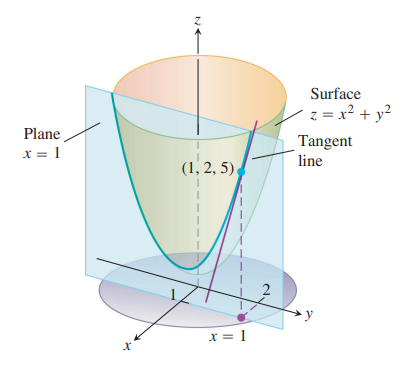
\includegraphics[scale=0.65]{example-6.1.3.png}
        \caption{The intersection of the plane $x=1$ and the paraboloid $z = x^2 + y^2$}
    \end{figure}

    The parabola formed at the intersection of $z = x^2 + y^2$ and $x = 1$ is $z = 1 + y^2$.
    The slope of the parabola so formed, at $(1, 3, 5)$ is:
    $$z_y \big|_{(1, 3, 5)} = 2y \big|_{(1, 3, 5)} = 6$$
\end{example}

\begin{example}
    \normalfont Given $f(x, y, z) = x \sin{(y + 3z)}$, find its partial derivative with respect to $z$.

    $$\frac{\del f(x, y, z)}{\del z} = f_z = 3x \cos{(y + 3z)}$$
\end{example}


\subsection{Higher-Order Partial Derivative}

\begin{enumerate}
     \item \textbf{Higher Partial Derivative} \\
    A $higher$ partial derivative is the partial derivative of a function with respect to the same variable multiple times.
    \begin{example}
        \normalfont $f_{xx},\ f_{yy},\ f_{xxx},\ f_{yyy},\ \hdots$
    \end{example}

    \item \textbf{Mixed Partial Derivative} \\
    A $mixed$ partial derivative is the partial derivative of a function with respect to different variables multiple times.
    \begin{example}
        \normalfont $f_{xy},\ f_{yx},\ f_{xxy},\ f_{xyx},\ f_{yyx},\ \hdots$
    \end{example}
\end{enumerate}

\begin{example}
    \normalfont Find the higher-order partial drivatives $f_{xy}$ and $f_{yx}$ for $f(x, y) = x\cos{y} + ye^x$.
    \begin{align*}
        f_x &= \cos{y} + ye^x &\ f_y &= -x\sin{y} + e^x \\
        f_{xy} &= -\sin{y} + e^x &\ f_{yx} &= -\sin{y} + e^x
    \end{align*}
\end{example}

\begin{theorem}
    [Mixed Derivative Theorem]
    If $f(x, y)$ and all its partial derivatives $f_x,\ f_y,\ f_{xy},$ and $f_{yx}$ are defined throughout an open region
    containing a point $\point \in \R^2$, and all are continuous at $\point$, then:
    \begin{equation}
        f_{xy}\point = f_{yx}\point.
    \end{equation}
\end{theorem}

\begin{example}
    \normalfont Find the second-order mixed partial derivative of $w(x, y) = xy + \frac{e^y}{y^2 + 1}$.
    \begin{align*}
        w_y &= x + \frac{1}{(y^2 + 1)^2} \left( \frac{e^y}{y^2 + 1} - \cdots \right) &\ w_x &= y + 0 \\
        w_{yx} &= 1 \text{ (as the term was a function of } y \text{)} &\ w_{xy} &= 1
    \end{align*}
\end{example}

\begin{theorem}
    [Increment Theorem for functions in two variables]
    In a region $R$ containing the point $\point$, the change in the value of the function $z = f(x, y)$ is given by
    \begin{equation}
        \Delta z = f(x_0 + \Delta x, y_0 + \Delta y) - f\point = (f_x \Delta x + f_y \Delta y) \big |_{\point}
    \end{equation}
\end{theorem}

\begin{theorem}
    [Chain Rule for more two variables]
    Provided that $w = f(x, y)$, and that $f_x$ and $f_y$ exist, then if $x = x(t)$ and $y = y(t)$, i.e. $x$ and $y$ are
    parametrized by $t$, then
    \begin{equation}
        \frac{dw}{dt} = f_x x_t + f_y y_t = \frac{\del f}{\del x} \frac{dx}{dt} + \frac{\del f}{\del y} \frac{dy}{dt}
    \end{equation}.
\end{theorem}

\begin{theorem}
    [Generalization of the Chain Rule]
    Provided that $w = f(x_1, x_2, \hdots, x_n)$, and that $f_{x_1}, f_{x_2}, \hdots, f_{x_n}$ exist, then if $x_i = x_i(t)$
    $\forall i \in \{1, 2, \hdots, n \}$, i.e. each $x_i$ is parametrized by $t$, then
    \begin{equation}
        \frac{dw}{dt} = \sum_{i=1}^n \frac{\del f}{\del x_i} \frac{dx_i}{dt}
    \end{equation}
\end{theorem}

\begin{example}
    \normalfont Find $w_t$ along $x = \sin{t}$ and $y = e^t$, given $w(x, y) = x^2y - y^2$.
    \begin{align*}
        w(t) &= e^t\sin^2{t} - e^{2t} &\ w(x, y) &= x^2y - y^2 \\
        w_t &= e^t\sin^2{t} + e^t\sin{2t} - 2e^{2t} &\ w_t &= 2xy(\cos{t}) + (x^2 - 2y)e^t \\
        &\ &\ w_t &= 2\sin{t}\cos{t} e^t + \sin^2{t} e^t - 2e^te^t \\
        &\ &\ w_t &= e^t\sin^2{t} + e^t\sin{2t} - 2e^{2t}
    \end{align*}
\end{example}


\subsection{Functions on a Surface}
A real-valued function in three variables is called a function on a \textit{surface}. Suppose the three variables, namely
$x, y, $ and $z$ are parametrized by $r$ and $s$. Then (say),

$$w = f(x, y, z);\text{ and } x = g(r, s),\ y = h(r, s), \text{ and } z = k(r, s)$$

Then,
\begin{align}
    \frac{dw}{dr} = \frac{\del f}{\del x} \frac{\del x}{\del r} + \frac{\del f}{\del y} \frac{\del y}{\del r} +
    \frac{\del f}{\del z} \frac{\del z}{\del r} = f_x x_r + f_y y_r + f_z z_r \\
    \frac{dw}{ds} = \frac{\del f}{\del x} \frac{\del x}{\del s} + \frac{\del f}{\del y} \frac{\del y}{\del s} +
    \frac{\del f}{\del z} \frac{\del z}{\del s} = f_x x_s + f_y y_s + f_z z_s
\end{align}

\begin{example}
    \normalfont Find $\frac{dw}{dr}$ if $w = x + 2y + z$, where $x = \frac{r}{s},\ y = r^2 + \text{ln}s$ and $z = 2r$.

    $$\frac{dw}{dr} = 1 \cdot \frac{1}{s} + 2 \cdot 2r + 1 \cdot 2 = \frac{1}{s} + 4r + 2$$
\end{example}

The same idea can be easily generalized to higher dimensions. Say, $w$ is a function of $n$-variables. Then,
$$w = f(x_1, x_2, \hdots, x_n); \text{ and } x_i = x_i(p_1, p_2, \hdots, p_m)$$

Then,
\begin{equation}
    \frac{dw}{dp_j} = \sum_{i = 1}^n f_{x_i} x_{i_{p_j}}, \text{ for some } 1 \leq j \leq m.
\end{equation}


\subsection{Implicit Differentiation}
Functions can be differentiated implictly to extract the rate of change of one variable with respect to another. However,
it is a tedious process.

\begin{theorem}
    [Formula for implicit differentiation]
    Suppose $F(x, y)$ is differentiable and that the equation $F(x, y) = 0$ defines $y$ as a differentiable function of $x$.
    Then, at any point where $f_y \neq 0$,
    \begin{equation}
        \frac{dy}{dx} = -\frac{F_x}{F_y}
    \end{equation}
\end{theorem}

\begin{example}
    \normalfont Find the derivative of $y$ with respect to $x$ given that $f(x, y) = y^2 - x^2 - \sin{(xy)} = 0$.
    $$\frac{dy}{dx} = -\frac{f_x}{f_y} = - \left( \frac{-2x - y\cos{(xy)}}{2y - x\cos{(xy)}} \right)
    = \frac{2x + y\cos{(xy)}}{2y - x\cos{(xy)}}$$
\end{example}

%%%%%%%%%%%%%%%%%%%%%%%%%%%%%%%%%%%%%%%%%%%%%%%%%%%%%%%%%%%%%%%%%%%%%%%%%%%%%%%%%%%%%%%%%%%%%%%%%%%%%%%%%%%%%%%%%%%%%%%%%%%%

% Directional Derivatives and Gradients
\section{Directional Derivatives and Gradients}

\subsection{Directional Derivatives}

The partial derivatives $f_x$ and $f_y$ of a function $z = f(x, y)$ are the rates of change of the output $z$ of along the
paths holding $y$ and $x$ constant, respectively. However, a derivative of a function can be found along any path.
The derivative of a function along a path other than one parallel to the axes is called the \textbf{directional derivative}.

The direction along which the derivative is calculated, is commonly notated by $\vec{u} = \langle u_1, u_2 \rangle$.

Formally, the derivative of a function $f(x, y)$ at a point $P_0 = \point$ in the direction of the unit vector
$\hat{u} = \langle u_1, u_2 \rangle$ is the number
\begin{equation}
    \left( \frac{df}{ds} \right)_{\hat{u}, P_0} = \ddvp = \lim_{s \to 0} \frac{f(x_0 + su_1, y_0 + su_2) - f\point}{s}
\end{equation}

provided the limit exists.

\textbf{Reference Link:}
\reference{https://www.youtube.com/watch?v=GJODOGq7cAY}{Directional Derivatives: What's the slope in any direction?}


\subsection{Gradients}

\subsubsection{Gradient of a function in two variables}
The gradient (gradient) of a function $f(x, y)$ is the vector $\langle f_x, f_y \rangle$.
\begin{equation}
    \grad f = \llangle \frac{\del f}{\del x}, \frac{\del f}{\del y} \rrangle = \langle f_x, f_y\rangle
\end{equation}
To evaluate the gradient at any particular point $P_0 = \point \in \R^2$, the partial derivatives need to be evaluated
at $P_0$.

\subsubsection{Gradient of a function in \texorpdfstring{$n$}{n} variables}
The gradient (gradient) of a function $f(x_1, x_2, \hdots, x_n)$ is the vector
$\langle f_{x_1}, f_{x_2}, \hdots, f_{x_n} \rangle$.
\begin{equation}
    \grad f = \llangle \frac{\del f}{\del x_1}, \frac{\del f}{\del x_2}, \hdots, \frac{\del f}{\del x_n} \rrangle
    = \langle f_x, f_y\rangle
\end{equation}
To evaluate the gradient at any particular point $P_0 = (x_{1_0}, x_{2_0}, \hdots, x_{n_0}) \in \R^n$, the partial
derivatives need to be evaluated at $P_0$.

\textbf{Reference Link:}
\reference{https://www.youtube.com/watch?v=QQPz3eXXgQI}{Geometric Meaning of the Gradient Vector}


\subsection{Relationship betwen Gradients and Directional Derivatives}
The directional derivative is essentially (just like any other derivative) the rate of change of a function. The only
For the directional derivative of a function $f(x, y)$ the input point $P_0 = \point$ is nudged along the line
parametrized by $s$.

Hence, given that $x = x_0 + su_1 \text{ and } y = y_0 + su_2,$
\begin{align*}
    \left( \frac{df}{ds} \right)_{\hat{u}, P_0} &= \frac{\del f}{\del x} \bigg|_{P_0} \frac{dx}{ds} +
    \frac{\del f}{\del y} \bigg|_{P_0} \frac{dy}{ds} \\
    &= \frac{\del f}{\del x} \bigg|_{P_0} u_1 + \frac{\del f}{\del y} \bigg|_{P_0} u_2 \\
    &= \langle f_x, f_y \rangle \cdot \langle u_1, u_2 \rangle \\
    &= (\grad f)_{P_0} \cdot \hat{u}
\end{align*}


\subsection{Directional Derivative as a Dot product}

\begin{theorem}
    [Directinal Derivative as a Dot product]
    If $f(x, y)$ is differentiable in an open region containing the point $P_0 = \point$, then
    \begin{equation}
        \left( \frac{df}{ds} \right)_{\hat{u}, P_0} = \ddvp = (\grad f)_{P_0} \cdot \hat{u}
    \end{equation}
\end{theorem}

\begin{example}
    \normalfont Find the directional derivative of $f(x, y) = x^2 \sin{2y}$ at $(1, \pi/2)$ along $\langle 3, -4 \rangle$.

    Given $P_0 = (1, \pi/2)$ and $\vec{u} = \langle 3, -4 \rangle \implies \hat{u} = \langle \frac{3}{5}, \frac{-4}{5} \rangle$
    \begin{align*}
        \grad f &= \llangle 2x \sin{2y},\ 2 x^2 \cos{2y} \rrangle \implies
        (\grad f)_{P_0} = \langle 0, 2\rangle \\
        \ddvp &= 0 \cdot \frac{3}{5} + 2 \cdot \frac{-4}{5} = 0 + \frac{-8}{5} = - \frac{8}{5}
    \end{align*}
\end{example}


\subsection{Direction of maximum, minimum, and zero change}

We can find the direction of extremum change of the function $f(x, y)$ by comparing the values of directional derivatives.
If $\theta$ is the angle between the gradient of $f$ at $P_0$ and the direction $\hat{u}$,
\begin{align*}
    \ddv &= \grad f \cdot \hat{u} \\
    \lVert \ddv \rVert &= \lVert \grad f \rVert\ \cos{\theta}
\end{align*}

And so the following three cases arise:
\begin{enumerate}
    \item $\theta = 0$: $\ddv$ is maximum, i.e. $\lVert \grad f \rVert$. $f$ increases the most rapidly
    when $\hat{u}$ is in the direction of $\grad f$.

    \item $\theta = \pi$: $\ddv$ is minimum, i.e. $- \lVert \grad f \rVert$. $f$ decreases the most rapidly
    when $\hat{u}$ is in the direction of $\grad f$.

    \item $\theta = \pi/2$: $\ddv = 0$, i.e. moving along $\hat{u}$ has no effect on $f$, i.e. the movement is along a contour.
\end{enumerate}

\begin{example}
    \normalfont Find the directions of maximum increase, maximum decrease, and zero change of
    $f(x, y) = \frac{x^2}{2} + \frac{y^2}{2}$ at the point $(1, 1)$.

    The gradient of the function at $(1, 1)$ is $(\grad f)_{(1, 1)} = \langle x, y \rangle_{(1, 1)} = \langle 1, 1\rangle$.

    \begin{enumerate}
        \item
        The function increases the most rapidly in the direction of $\grad f$. Therefore, the direction of maximum increase is
        $$\hat{u} = \llangle \frac{1}{\sqrt{2}}, \frac{1}{\sqrt{2}} \rrangle =
        \frac{1}{\sqrt{2}} \hat{i} + \frac{1}{\sqrt{2}} \hat{j}$$

        \item
        The function decreases the most rapidly in the direction opposite to $\grad f$. Therefore, the
        direction of maximum decrease is
        $$\hat{u} = \llangle -\frac{1}{\sqrt{2}}, -\frac{1}{\sqrt{2}} \rrangle =
        -\frac{1}{\sqrt{2}} \hat{i} - \frac{1}{\sqrt{2}} \hat{j}$$

        \item
        The direction of zero change are the directions orthogonal to $\grad f$. There are
        $$\hat{n} = \llangle \frac{1}{\sqrt{2}}, -\frac{1}{\sqrt{2}} \rrangle =
        \frac{1}{\sqrt{2}} \hat{i} -\frac{1}{\sqrt{2}} \hat{j} \text{ and }
        -\hat{n} = \llangle - \frac{1}{\sqrt{2}}, \frac{1}{\sqrt{2}} \rrangle =
        -\frac{1}{\sqrt{2}} \hat{i} + \frac{1}{\sqrt{2}} \hat{j}$$
    \end{enumerate}
\end{example}


\subsection{Properties of the Gradient}
The following algebraic rules are obeyed by gradients. The rules are similar to the algebra derivatives (notice the
difference in the \textbf{Quotient Rule}):

\begin{enumerate}
    \item \textbf{Scaling Rule:} $\grad (kf) = k \grad f$
    \item \textbf{Sum/Difference Rule:} $\grad (f \pm g) = \grad f \pm \grad g$
    \item \textbf{Product Rule:} $\grad (fg) = f \grad g + g \grad f$
    \item \textbf{Quotient Rule:} $\grad \left( \frac{f}{g} \right) = \frac{g\grad f - f\grad g}{g^2}$
\end{enumerate}

%%%%%%%%%%%%%%%%%%%%%%%%%%%%%%%%%%%%%%%%%%%%%%%%%%%%%%%%%%%%%%%%%%%%%%%%%%%%%%%%%%%%%%%%%%%%%%%%%%%%%%%%%%%%%%%%%%%%%%%%%%%%

% Tangents and Normals
\section{Tangents and Normals}

\subsection{Tangent Lines to Level Curves}

If $\vec{r} = g(t)\hat{i} + h(t)\hat{j}$ is a smooth curve on the level curve $f(x, y) = c$ of a differentiable function $f$, then
\begin{align*}
    f(g(t), h(t)) &= c \\
    \frac{d}{dt} f(g(t), h(t)) &= \frac{d}{dt}(c) \\
    \frac{\del f}{\del x} \frac{dg}{dt} + \frac{\del f}{\del y} \frac{dh}{dt} &= 0 \\
    \llangle \frac{\del f}{\del x}, \frac{\del f}{\del y} \rrangle \cdot \llangle \frac{dg}{dt}, \frac{dh}{dt} \rrangle &= 0 \\
    \grad f \cdot \frac{d\vec{r}}{dt} &= 0
\end{align*}

This essentially means that the gradient of $f$ is always normal to the tangent at a level curve, which makes sense as
gradient describes the change, whereas the level curve describes the \textit{constant-ness}.

The line through a point $P_0 = \point$ normal to a vector $\vec{n} = A\hat{i} + B\hat{j}$ has the equation
\begin{equation}
    A(x - x_0) + B(y - y_0) = 0
\end{equation}

And if $\vec{n}$ is the gradient $(\grad f)_{\point} = f_x\point\hat{i} + f_y\point\hat{j}$,
the equation of the tangent line is given by
\begin{equation}
    f_x\point (x - x_0) + f_y \point (y - y_0) = 0
\end{equation}

\begin{example}
    \normalfont Find the equation of the tangent to the given ellipse at $(-2, 1)$.
    $$\frac{x^2}{4} + y^2 = 2$$

    Note that the given ellipse is a level curve of $f(x, y) = \frac{x^2}{4} + y^2$. Then, at $(-2, 1)$,
    $$ (\grad f)_{(2, -1)} = \llangle \frac{x}{2}, 2y \rrangle_{(-2, 1)} = \langle -1, 2 \rangle $$

    Hence, the tangent to the ellipse at $(-2, 1)$ is given by
    \begin{align*}
        -1 (x - (-2)) + 2 (y - 1) &= 0 \\
        x - 2y &= -4
    \end{align*}
\end{example}


\subsection{Tangent Planes to Level Surfaces}
If $\vec{r} = g(t)\hat{i} + h(t)\hat{j} + k(t)\hat{k}$ is a smooth curve on the level urface $f(x, y, z) = c$ of a differentiable
function $f$, then
\begin{align*}
    f(g(t), h(t), k(t)) &= c \\
    \frac{d}{dt} f(g(t), h(t), k(t)) &= \frac{d}{dt}(c) \\
    \frac{\del f}{\del x} \frac{dg}{dt} + \frac{\del f}{\del y} \frac{dh}{dt} + \frac{\del f}{\del z} \frac{dk}{dt} &= 0 \\
    \llangle \frac{\del f}{\del x}, \frac{\del f}{\del y}, \frac{\del f}{\del z} \rrangle \cdot
    \llangle \frac{dg}{dt}, \frac{dh}{dt}, \frac{dk}{dt} \rrangle &= 0 \\
    \grad f \cdot \frac{d\vec{r}}{dt} &= 0
\end{align*}

Analagous to \textit{tangent lines to level curves}, this means that the tangent at a level curve is always normal to the
gradient at any point. So, if $\vec{n}$ is the gradient $(\grad f)_{P_0} = f_x(P_0)\hat{i} + f_y(P_0)\hat{j} + f_z(P_0)\hat{k}$
for some $P_0 = (x_0, y_0, z_0) \in \R^3$, then the equation of the tangent plane is given by

\begin{equation}
    f_x(P_0)(x - x_0) + f_y(P_0)(y - y_0) + f_z(P_0)(z - z_0) = 0
\end{equation}

Thus, the tangent plane at a point $P_0$ on the level surface $f(x, y, z) = c$ is a plane normal to $(\grad f)_{P_0}$.


\subsection{Normal Line to Level Curves and Surfaces}
The normal line to a level curve $f(x, y) = c$ at a point $P_0 = \point \in \R^2$, or to a level surface $f(x, y, z) = c$ at a point
$P_0 = (x_0, y_0, z_0) \in \R^3$, is a line through $P_0$ parallel to $(\grad f)_{P_0}$. In three dimensions, the equation
of the normal is given by

$$x = x_0 + f_x(P_0) t, \ \ \ y = y_0 + f_y(P_0) t, \ \ \ z = z_0 + f_z(P_0) t$$

\begin{figure}[htp]
    \centering
    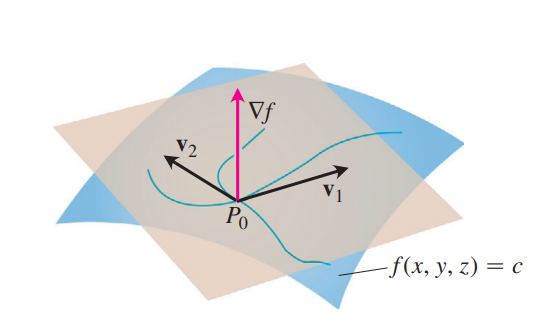
\includegraphics[scale=0.45]{tangent-normal.png}
    \caption{The gradient $\grad f$ is orthogonal to the tangent plane of a level surface}
\end{figure}

\begin{example}
    \normalfont Find the tangent plane and normal line of the surface $f(x, y, z) = x^2 + y^2 + z - 9 = 0$ at the point
    $P_0 = (1, 2, 4)$.

    We first find the gradient of $f$:
    $$(\grad f)_{P_0} = \langle 2x, 2y, 1 \rangle_{P_0} = \langle 2, 4, 1\rangle$$

    Hence, the equation of the tangent plane is
    \begin{align*}
        2 (x - 1) + 4 (y - 2) + 1 (z - 4) &= 0 \\
        2x + 4y + z &= 14
    \end{align*}

    For the equation of the normal line at $P_0$, we have
    $$\frac{x - 1}{2} = \frac{y - 2}{4} = z - 4$$
\end{example}

\begin{example}
    \normalfont The surfaces $f(x, y, z) = x^2 + y^2 - 2 = 0$ (a cylinder) and $f(x, y, z) = x + z - 4 = 0$ (a plane)
    meet in an ellipse $E$. Find the parametric equations for the line tangent to $E$ at $P_0 = (1, 1, 3)$.

    \begin{figure}[htp]
        \centering
        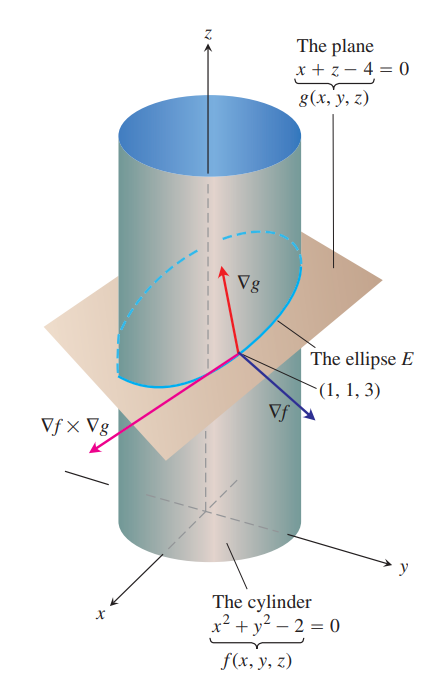
\includegraphics[scale=0.5]{example-8.3.2.png}
        \caption{Intersection of Cylinder $f(x, y, z) = 0$ and Plane $g(x, y, z) = 0$}
    \end{figure}

    Note that the tangent to $E$ is orthogonal both to the gradient of the cylinder, $\grad f$, and the gradient
    of the plane, $\grad g$. Hence, the tangent is parallel to $\vec{v} = \grad f \times \grad g$.

    \begin{align*}
        (\grad f)_{P_0} &= \langle 2x, 2y, 0 \rangle_{P_0} = \langle 2, 2, 0 \rangle \\
        (\grad g)_{P_0} &= \langle 1, 0, 1 \rangle_{P_0} = \langle 1, 0, 1\rangle \\
        \vec{v} &= \langle 2, 2, 0 \rangle \times \langle 1, 0, 1 \rangle =
        \begin{vmatrix}
            \hat{i} & \hat{j} & \hat{k} \\
            2 & 2 & 0 \\
            1 & 0 & 1
        \end{vmatrix} = 2\hat{i} - 2\hat{j} - 2\hat{k}
    \end{align*}

    Hence, the parametric equation of the line is
    $$x = 1 + 2t, \ y = 1 - 2t, \ z = 3 - 2t, \text{  or  } \vec{r} = (\hat{i} + \hat{j} + 3\hat{j}) +
    \lambda (\hat{i} - \hat{j} - \hat{k})$$
\end{example}

%%%%%%%%%%%%%%%%%%%%%%%%%%%%%%%%%%%%%%%%%%%%%%%%%%%%%%%%%%%%%%%%%%%%%%%%%%%%%%%%%%%%%%%%%%%%%%%%%%%%%%%%%%%%%%%%%%%%%%%%%%%%

% Approximations, Linearization, and Total Differentials
\section{Approximation, Linearization, and Total Differentials}

\subsection{Estimating change in a Specific Direction}
To estimate how much the value of a differential function $f$ changes if we move a small distance $ds$ from a point $P_0$
in a direction $\hat{u}$, the following formula is used:

\begin{equation}
    df = (\grad f \big|_{P_0} \cdot \hat{u}) \cdot ds
\end{equation}

\begin{example}
    \normalfont Estimate how much the value of $f(x, y, z) = y \sin{x} + 2yz$ will change if the point $P = (x, y, z)$
    moves 0.1 units from $P_0(0, 1, 0)$ straight towards $P_1(2, 2, -2)$.

    First, we find out the direction of movement
    \begin{align*}
        \vec{u} &= \langle 2-0, 2-1, -2-0 \rangle = \langle 2, 1, -2 \rangle \\
        \implies \hat{u} &= \llangle \frac{2}{3}, \frac{1}{3}, -\frac{2}{3} \rrangle
    \end{align*}

    The gradient of $f$ at $P_0$ is
    $$\grad f \big|_{P_0} = \langle y \cos{x}, \sin{x} + 2z, 2y \rangle_{P_0} = \langle 1, 0, 2 \rangle$$

    Therefore, estimated change $df$ on moving $ds = 0.1$ units in the direction of $\hat{u}$ will be
    \begin{align*}
        df &= (\grad f \big|_{P-0} \cdot \hat{u}) \cdot ds \\
        &= \left( \langle 1, 0, 2 \rangle \cdot \llangle \frac{2}{3}, \frac{1}{3}, -\frac{2}{3} \rrangle \right) \times 0.1 \\
        &= -\frac{2}{3} \times 0.1 \approx -0.067 \text{ units }
    \end{align*}
\end{example}


\subsection{Linearization}

\textbf{Linearization} is a linear approximation of a function near some specific point. The linearization of a function
$f(x, y)$ at a point $\point$ where $f$ is differentiable is the function

\begin{equation}
    L(x, y) = f\point + f_x \point (x - x_0) + f_y \point (y - y_0)
\end{equation}

and the approximation $f(x, y) \approx L(x, y)$ is called the \textbf{standard linear approximation} of $f$ at $\point$.

The plane $z = L(x, y)$ is tangent to the surface $z = f(x, y)$ at the point $\point$. This is because the tangent plane is a
good approximation for the function near the point of contact. Thus, linearization of a function in two variables is a tangent
plane, and the linearization of a function in one variable is a tangent line.

\begin{example}
    \normalfont Find the linearization of $f(x, y) = x^2 - xy + \frac{y^2}{2} + 3$ at the point $(3, 2)$.

    First, we find $f(3, 2), f_x(3, 2), $ and $f_y(3, 2)$
    \begin{align*}
        f(3, 2) &= 9 - 6 + 2 + 3 = 8 \\
        f_x(3, 2) &= (2x - y)_{(3, 2)} = 6 - 2 = 4 \\
        f_y(3, 2) &= (-x + y)_{(3, 2)} = -3 + 2 = -1
    \end{align*}

    Then, the linear approximation of $f$ at $(3, 2)$ will be given by
    \begin{align*}
        L(x, y) &= 8 + 4(x - 3) - 1(y - 2) \\
        &= 4x - y - 2
    \end{align*}
\end{example}


\subsection{Error in Linearization}

The absolute error in linearization is the difference in of the functions $f(x, y)$ and $L(x, y)$, i.e.
\begin{equation}
    E(x, y) = f(x, y) - L(x, y)
\end{equation}

If $f$ has continuous first and second partial derivatives throughout the region containing $\point$, and if $M$ is an
upper bound for the values of $f_{xx}, f_{yy},$ and $f_{xy}$ in the region, then the error $E(x, y)$ satisfies the
following inequality:
\begin{equation}
    |E(x, y)| \leq \frac{1}{2} M (|x - x_0| + |y - y_0|)^2
\end{equation}

\begin{example}
    \normalfont Find an upper bound for the error in the approximation $f(x, y) \approx L(x, y)$ derived in
    \textbf{Example 9.2.1} over the rectangle $R: |x - 3| \leq 0.1, |y - 2| \leq 0.1$, as a percentage of $f(3, 2)$.

    We begin by calculating $f_{xx}, f_{yy},$ and $f_{xy}$
    $$|f_{xx}| = |2| = 2, \ \ \ |f_{yy}| = |-1| = 1, \ \ \ |f_{xy}| = |1| = 1$$

    Therefore, $M$ can be assigned $\max{\{f_{xx}, f_{yy}, f_{xy}\}} = 2$. Then, given that $|x - 3| \leq 0.1$ and
    $|y - 2| \leq 0.1$,
    \begin{align*}
        |E(x, y)| &\leq \frac{1}{2} (2) (|x - 3| + |y - 2|)^2 \\
        &\leq (0.1 + 0.1) ^ 2 = 0.04
    \end{align*}

    Hence, the upper bound for the error in linearization is $0.04$, and as a percentage of $f(3, 2)$, is
    $$\frac{0.04}{8} \times 100 = 5 \%$$
\end{example}


\subsection{Total Differentials}
The \textbf{differential} of a function is the change in its value for very little changes in its inputs. So, if we move
from a point $\point$ to a point $(x_0 + dx, y_0 + dy)$, the resulting change (differential) is
\begin{equation}
    df = \Delta f \big|_{\point} = f_x \point dx + f_y \point dy
\end{equation}

This change $df$ in the linearization of $f$ is called its \textbf{total differential}.

\begin{example}
    \normalfont Suppose that a cylinder is designed to have a radius of 1 in. and a height of 5 in., but that the radius
    and height are off by $dr = +0.03$ and $dh = -0.1$. Estimate the resulting change in volume.

    For the volume of a cylinder, we have
    \begin{align*}
        V &= \pi r^2 h \\
        \Delta V \approx dV &= V_r(r_0, h_0) dr + V_h(r_0, h_0) dh
    \end{align*}

    Note that $V_r = 2 \pi r h$ and $V_h = \pi r^2$. Then
    \begin{align*}
        dV &= 2 \pi \cdot 1 \cdot 5 (0.03) + \pi \cdot 1^2 (-0.1) \\
        &= 0.3 \pi - 0.1 \pi = 0.2 \pi \approx 0.63 \text{ in.}^3
    \end{align*}
\end{example}

\begin{example}
    \normalfont The percentage errors in measured radius and height of a cylinder are no more than 2\% and 0.5\%
    respectively. Estimate the percentage error in calculation of its volume.

    Given that
    $$\left| \frac{dr}{r} \times 100 \right| \leq 2 \ \ \ \text{ and } \ \ \
    \left| \frac{dh}{h} \times 100 \right| \leq 0.5$$

    Then,
    \begin{align*}
        \frac{dV}{V} &= \frac{2 \pi r h\ dr + \pi r^2\ dh}{\pi r^2 h} = \frac{2dr}{r} + \frac{dh}{h} \\
        \left| \frac{dV}{V} \right| &\leq 2 \left| \frac{dr}{r} \right| + \left| \frac{dh}{h} \right| \\
        &\leq 2 (0.02) + 0.005 = 0.045
    \end{align*}
\end{example}


\subsection{Extension to three dimensions}
Analogous to two dimensions, the following hold in three dimensions:

\begin{enumerate}
    \item
    The linearization of a function $f(x, y, z)$ at a point $P_0 = (x_0, y_0, z_0)$ is given by
    \begin{equation}
        L(x, y, z) = f(P_0) + f_x(P_0)(x - x_0) + f_y(P_0)(y - y_0) + f_z(P_0)(z - z_0)
    \end{equation}

    \item
    Let $R$ is a rectangular region centered at $P_0$, where the partial derivates of $f$ are continuous. Suppose throughout
    $R$, the magnitude of all second derivates of $f$ are less than or equal to $M$. Then, the error
    $E(x, y, z) = f(x, y, z) - L(x, y, z)$ in the approximation of $f$ is
    \begin{equation}
        |E| \leq \frac{1}{2}M (|x - x_0| + |y - y_0| + |z - z_0|)^2
    \end{equation}

    \item
    If the second partial derivatives of $f$ are are continuous, and if $x, y,$ and $z$ change from
    $x_0, y_0,$ and $z_0$ by small amounts $dx, dy,$ and $dz$, the total differential (estimated change) is
    \begin{equation}
        df = f_x(P_0) dx + f_y(P_0) dy + f_z(P_0) dz
    \end{equation}
\end{enumerate}

%%%%%%%%%%%%%%%%%%%%%%%%%%%%%%%%%%%%%%%%%%%%%%%%%%%%%%%%%%%%%%%%%%%%%%%%%%%%%%%%%%%%%%%%%%%%%%%%%%%%%%%%%%%%%%%%%%%%%%%%%%%%

% Extreme Values, Critical Points, and Saddle Points
\section{Extreme Values, Critical Points, and Saddle Points}

To find the local extremum of a function in one variable, we look for points on its graph having a horizontal tangent line.
The local extrema are also called \textbf{relative extrema}.

\subsection{Local Extremum}
Let $f(x, y)$ be defined on a region $R$ containing the point $(a, b)$. Then,

\begin{enumerate}
    \item $f(a, b)$ is a \textbf{local maximum} value of $f$ if $f(a, b) \geq f(x, y)$ for all domain points $(x, y)$ in an
    open disk centered at $(a, b)$.

    \item $f(a, b)$ is a \textbf{local minimum} value of $f$ if $f(a, b) \leq f(x, y)$ for all domain points $(x, y)$ in an
    open disk centered at $(a, b)$.
\end{enumerate}

Local maxima correspond to \textit{mountain peaks} on the surface $z = f(x, y)$, whereas local minima correspond to
\textit{valley bottoms}.

\begin{theorem}[First Derivative Test]
    If $f(x, y)$ has a local extremum at an interior point $(a, b)$ of its domain and if the first partial derivatives exist
    there, then $f_x(a, b) = f_y(a, b) = 0$.
\end{theorem}


\subsection{Critical Point}
An interior point of the domain of a function $f(x, y)$ where both $f_x$ and $f_y$ are zero, or where one or both of $f_x$
and $f_y$ do not exist is a \textbf{critical point} of $f$.

\textbf{Theorem 7} essentially says that a function $f(x, y)$ can only assume extreme values at critical points or boundary
points. But not every critical point gives rise to a local extremum. A differentiable function of one variable may have a
\textit{point of inflection}, whereas a differentiable function in two variables might have a \textit{saddle point}.

\begin{example}
    \normalfont Find the local extreme values of $f(x, y) = x^2 + y^2$.

    We find the gradient of the function, $\grad f = \langle 2x, 2y \rangle$. The partial derivatives are 0 at $(0, 0)$.
    Since $f$ is never negative, the origin is the local minimum.
\end{example}


\subsection{Saddle Point}
A critical point $(a, b)$ where in every open disk centered at $(a, b)$, there are domain points where $f(x, y) > f(a, b)$
and domain points where $f(x, y) < f(a, b)$ is called a \textbf{saddle point} $(a, b, f(a, b))$ of the surface
$z = f(x, y)$.

\begin{example}
    \normalfont Find the local extreme values of $f(x, y) = y^2 - x^2$.

    We find that the partial derivatives of $f$ are $f_x = -2x$ and $f_y = 2y$. Both the parital derivatives are 0 at the origin.
    However, note that $f(x, 0) = -x^2 < 0 (for x > 0)$, and $f(0, y) = y^2 > 0 (for y > 0)$. Hence, the origin is a saddle point.
\end{example}

\begin{theorem}[Second Derivative Test]
    Suppose that $f(x, y)$ and its first and second partial derivatives are continuous throughout a disk centered at $(a, b)$, and
    that $f_X(a, b) = f_y(a, b) = 0$. Then
    \begin{enumerate}
        \item $f$ has a \textbf{local maximum} at $(a, b)$ if $f_{xx} < 0$ and $f_{xx}f_{yy} - f{xy}^2 > 0$ at $(a, b)$.
        \item $f$ has a \textbf{local minimum} at $(a, b)$ if $f_{xx} > 0$ and $f_{xx}f_{yy} - f{xy}^2 > 0$ at $(a, b)$.
        \item $f$ has a \textbf{saddle point} at $(a, b)$ if $f_{xx}f_{yy} - f{xy}^2 < 0$ at $(a, b)$.
        \item The test is inconclusive at $(a, b)$ if $f_{xx}f_{yy} - f{xy}^2 = 0$.
    \end{enumerate}
\end{theorem}


\subsection{Discriminant or Hessian of \texorpdfstring{$f$}{f}}
The expression $f_{xx}f_{yy} - f_{xy}^2$ is called the \textbf{discriminant} or \textbf{Hessian} of f.
\begin{equation}
    f_{xx}f_{yy} - f_{xy}^2 =
    \begin{vmatrix}
        f_{xx} & f_{xy} \\ f_{yx} & f_{yy}
    \end{vmatrix}
\end{equation}

\textbf{Theorem 8} essentially says that if the discriminant is positive, the surface curves the same way in all directions.
If $f_{xx} < 0$, then it curves downwards, giving rise to local maxima, and vice-versa. And if the discriminant is negative,
then it curves upwards in some directions and downwards in others.

\begin{example}
    \normalfont Find the local extreme points of $f(x, y) = xy$.

    \begin{figure}[htp]
        \centering
        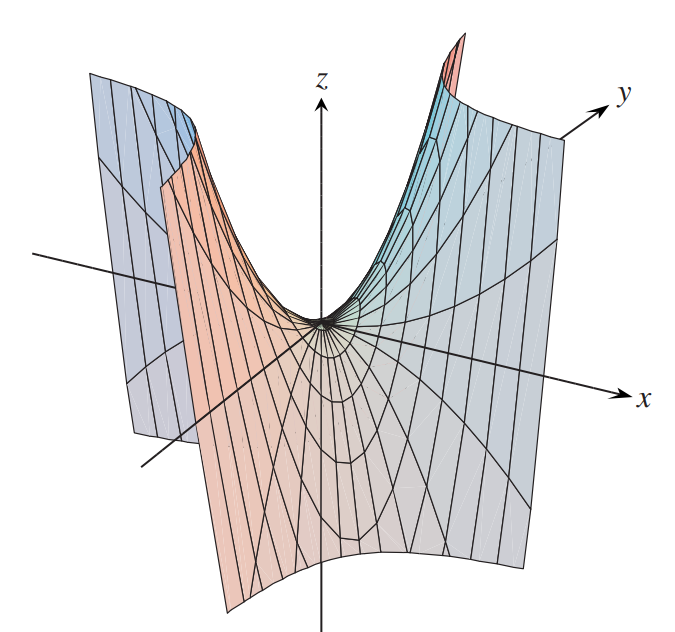
\includegraphics[scale=0.35]{saddle-point.png}
        \caption{The surface $z = xy$}
    \end{figure}

    Since $f$ is differentiable everywhere, its critical points can occur only where
    $$f_x = y = 0 \ \ \ \text{and} \ \ \ f_y = x = 0$$

    This only happens at $(0, 0)$. Next, we find the double partial derivatives
    $$f_{xx} = 0, \ \ \ f_{yy} = 0, \ \ \ f_{xy} = 1$$

    Hence, the discriminant becomes $f_{xx}f_{yy} - f{xy}^2 = -1 < 0$, and hence, the origin is a saddle point.
    Since there are no other critical points, the function does not have a local extremum.
\end{example}


\subsection{Absolute Extrema on Closed Bounded Regions}
Absolute extrema of a continuous function $f(x, y)$ on a closed bounded region $R$ are found in three steps:
\begin{enumerate}
    \item List down the critical points of $f$ and evaluate $f$ at these points.
    \item List down the boundary points of $f$ where it has local maxima/minima and evaluate $f$ at these points.
    \item The maximum value of $f$ in this list is the absolute maxima of $f$ on $R$, and the minimum value is the
    absolute minima.
\end{enumerate}

\begin{example}
    \normalfont Find the absolute maximum and minimum values of $f(x, y) = 2 + 2x + 2y - x^2 - y^2$ on the triangular
    region bounded by $x = 0, y = 0, y = 9 - x$.

    First, we find the critical points of $f$.
    $$f_x = 2 - 2x = 0 \ \ \ \text{ and } \ \ \ f_y = 2 - 2y = 0$$
    which gives the point $(1, 1)$. $f(1, 1) = 4$.

    For the boundary points, we have (for):
    \begin{enumerate}
        \item
        $$y = 0 \implies f(x, 0) = 2 + 2x - x^2$$
        The absolute extrema for this function can occur at its end-points, and in the interior where its derivative is 0.
        $f'(x, 0) = 2 - 2x = 0 \implies x = 1$. \\
        Therefore, $f(0, 0) = 2, f(9, 0) = -61, f(1, 0) = 3$.

        \item
        $$x = 0 \implies f(0, y) = 2 + 2y - y^2$$
        The absolute extrema for this function can occur at its end-points, and in the interior where its derivative is 0.
        $f'(0, y) = 2 - 2y = 0 \implies y = 1$. \\
        Therefore, $f(0, 0) = 2, f(0, 9) = -61, f(0, 1) = 3$.

        \item
        $$y = 9 - x \implies f(x, 9-x) = -61 + 18x - 2x^2$$
        The absolute extrema for this function can occur at the interior points where its derivative is 0.
        $f'(x, 9-x) = 18 - 4x = 0 \implies x = \frac{9}{2}$. \\
        Therefore, $f(\frac{9}{2}, 9-\frac{9}{2}) = -\frac{41}{2}$.
    \end{enumerate}
\end{example}

%%%%%%%%%%%%%%%%%%%%%%%%%%%%%%%%%%%%%%%%%%%%%%%%%%%%%%%%%%%%%%%%%%%%%%%%%%%%%%%%%%%%%%%%%%%%%%%%%%%%%%%%%%%%%%%%%%%%%%%%%%%%

\end{document}